\chapter{Python Excel Integration}\label{ch:python-excel-integration}

The use of Microsoft Excel in financial institutions practising
Quantitative Analysis is simply too widespread to be
overlooked. Python, or more specifically, the Win32 Python extensions,
make it easy to access Python functionality from Microsoft Excel. To
do so, we dip into the world of COM\footnote{COM is an acronym
standing for the ``Component Object Model'', a (partially
standardised) technology from the Microsoft Windows family of
operating systems.}. We won't attempt to teach COM here, it's too
broad a subject for this book, but will instead focus on how we can
write simple COM servers in Python and COM clients in Microsoft Excel
VBA\footnote{VBA is an acronym for ``Visual Basic for
Applications''}. For richer details regarding Python/COM integration
beyond those presented here, readers are strongly recommended to consult
Hammond \& Robinson's ``Python Programming on
Win32''\cite{book:HAMMOND}. For those readers who are interested in acquiring a
deeper understanding of COM beyond the specific field of Python/COM
integration we recommend Don Box's ``Essential
COM''\cite{book:BOX}.

\section{Black-Scholes COM server}\label{sec:black-scholes-com-server}

To illustrate the basic ideas of publishing COM servers in Python
we'll jump straight in with a COM component exposing the functionality
of the \\
\verb|ppf.core.black_scholes| module. The code presented below can be
found in the \verb|ppf.com.black_scholes| module.

\begin{verbatim}
class BlackScholes:
  _public_methods_ = ["OptionPrice"]
  _reg_clsid_ = "{14B40B3E-DC9A-4E07-A512-F65DA07BDC09}"
  _reg_progid_ = "ppf.black_scholes"

  def OptionPrice(self, spot, strike, rate, vol, time, call_put):
     from win32com.server.exception import COMException
     from ppf.core import black_scholes
     try:
       return black_scholes(
         S=spot, K=strike, r=rate, sig=vol, T=time, CP=call_put)
     except RuntimeError, e:
       raise COMException(
            desc="ppf error : \""+str(e)+"\"", scode=0x80040201)

if __name__ == "__main__":
  print "Registering \"BlackScholes\" server... ",
  import win32com.server.register
  win32com.server.register.UseCommandLine(BlackScholes)
  print  "done!"
\end{verbatim}

The first thing to note about the code above is that the Black-Scholes
COM server is really nothing more than a decorated Python class. The
Python Win32 framework does most of the work that relates to COM
specifically (argument conversions between the Win32 \verb|VARIANT|
data-type and native Python data-types for example). The \verb|class BlackScholes|
COM component exposes one function, \verb|OptionPrice|
which is a wrapper around the \verb|ppf.core.black_scholes|
function. The intention of publishing the \verb|OptionPrice| function
in the \verb|BlackScholes| interface is expressed by adding the name
of the function to the class static data member
\verb|_public_methods_|. Although not shown here, additional
functions that the class may have, unless added to this list, will not
form part of the COM interface offered by the class. In COM, class IDs
(CLSID) are 128-bit globally unique identifiers (GUID) associated with
COM objects. The \verb|_reg_clsid_| class data member assigns to our
\verb|class BlackScholes| the value \emph{`{14B40B3E-DC9A-4E07-A512-F65DA07BDC09}'}
. These CLSIDs should never be copied. Instead they can and should be
generated for each new COM component developed in the following way:
\begin{verbatim} 
>>> import pythoncom
>>> print str(pythoncom.CreateGuid())
{1C8D8011-01D9-492A-974B-7B5CE3F3DF43}
\end{verbatim}
In addition to naming COM objects by their CLSIDs, COM allows for
text-based aliases called programmatic IDs or ProgIDs. These are
usually in the form \emph{libraryname.classname.version}. Our
\verb|class BlackScholes| is assigned the ProgID given by the value of
the \verb|_reg_progid_| class variable, that is,\\
\emph{`ppf.black\_scholes'}.

If run from the command line, the \verb|__main__| function takes care
of registering the \verb|BlackScholes| component with COM. We'll skip
the details of precisely what that involves and ultimately means but
in short, a collection of values are written to the Windows registry
based on the information provided by the class data members just
covered that enables operating system calls at run-time to discover
our \verb|BlackScholes| class and allow instances of them to be
created in the calling process (COM (late-bound automation) clients --
we'll get on to examples in just a moment).
\begin{figure}
\centering
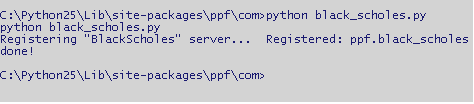
\includegraphics[scale=0.5]{img/register_server.PNG}
\caption{Registering the PPF Black-Scholes COM server.}
\end{figure}

Before we present an automation client that exercises the
functionality provided by our \verb|BlackScholes| component, we'll
quickly cover the definition of the \verb|OptionPrice| function. As
noted earlier, it's a simple wrapper around the
\verb|ppf.core.black_scholes| function. One important responsibility
of the wrapper is to trap any Python exceptions that may result from
the call to the \verb|ppf.core.black_scholes| function and translate
them into\\ \verb|win32.com.server.exception.COMException| exception
objects. The Python COM framework takes charge of phrasing such
exceptions in terms the calling environment (automation clients,) can
deal with. This is important since such environments will in general
know nothing about how to deal with raw Python exceptions (in fact,
the code
\begin{verbatim}
     raise COMException(
          desc="ppf error : \""+str(e)+"\"", scode=0x80040201)
\end{verbatim}
is creating a \verb|COMException| with a custom error
code. This works around a VB6 bug(?) and makes sure the text of the
the exception, detailing the \verb|ppf| error, is made available to
the calling client.)

\subsection{VBS client}

COM is all about getting objects in different languages talking to
each other. We'll put that to the test right now by implementing a
client of the \verb|BlackScholes| server from the preceding section
in Microsoft VBScript that is intended to be executed under the
Microsoft Windows Scripting Host environment offered by the command
line interpreter \verb|cscript.exe|. The code can be found in the
`example' directory of the code accompanying the book in the file
`test\_black\_scholes.vbs'.
\begin{verbatim}
On Error Resume Next

Dim Pricer : Set Pricer = CreateObject("ppf.black_scholes")
Dim spot: spot = 42.
Dim strike: strike = 40.
Dim r: r = 0.1
Dim sig: sig = 0.2
Dim T: T= 0.5
Dim european_call: european_call = 1

Dim price : price = Pricer.OptionPrice(spot, strike, r, sig, T, european_call)

If Err.Number <> 0 Then
  WScript.Echo "Automation error : " & vbCr & Err.Number & _
               " (" & Hex(Err.Number) & ")" & vbCr & Err.Description
  Err.Clear
Else
  WScript.Echo price
End If

Set Pricer = Nothing
\end{verbatim}
Figure \ref{fig:invoke-black-scholes-from-vbs} shows the result of
executing the client script.
\begin{figure}
\centering
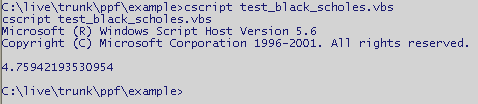
\includegraphics[scale=0.5]{img/black_scholes_vbs_client.PNG}
\caption{Invoking the PPF Black-Scholes function from VBScript.}
\label{fig:invoke-black-scholes-from-vbs}
\end{figure}

\subsection{VBA client}

The following Microsoft Excel VBA code implements a Black-Scholes
client suitable for use in Microsoft Excel. Figure
\ref{fig:invoke-black-scholes-from-vba} shows an example session
exercising the client on an Excel worksheet.
\begin{verbatim}
Public Function PPF_BlackScholes( _
   Spot As Double, _
   Strike As Double, _
   Rate As Double, _
   Vol As Double, _
   T As Double, _
   CallPut As Double) As Variant
  On Error Resume Next
  Dim Pricer As Object: Set Pricer = CreateObject("ppf.black_scholes")
  PPF_BlackScholes = Pricer.OptionPrice(Spot, Strike, Rate, Vol, T, CallPut)
  If Err.Number <> 0 Then
    PPF_BlackScholes = "#err: " & Err.Description
    Err.Clear
  End If
  Set Pricer = Nothing
End Function
\end{verbatim}
\begin{figure}
\centering
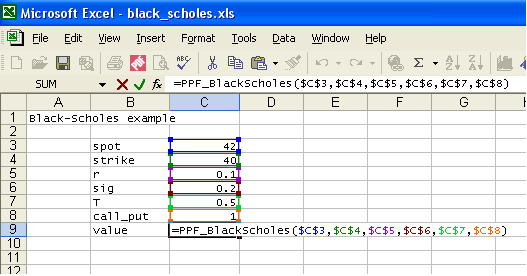
\includegraphics[scale=0.5]{img/black_scholes.PNG}
\caption{Invoking the PPF Black-Scholes function from Microsoft Excel.}
\label{fig:invoke-black-scholes-from-vba}
\end{figure}

\section{Numerical Pricing with PPF in Excel}

Armed with the understanding of the basic principles of publishing
Python COM components from the preceding section, we now consider how
we can assemble such components into a broader example to provide
numerical pricing capabilities using PPF in Excel. Specifically, our
goal will be to enable Bermudan swaption pricing on a Hull-White
lattice.

\subsection{Common utilities}

Before going on, we will find in implementing the COM servers for this
example some code that is common amongst all the servers that it is
helpful to factor out (to aid clarity and reduce unnecessary code
repetition). The simple utilities presented here all reside in the the
\verb|ppf.com.utils| module.

\subsubsection{Date conversion}

The \verb|to_ppf_date| function converts a Win32 COM date into a
\verb|ppf.date_time.date| representation. It is frequently used at the
boundary between the COM servers and `pure' \verb|ppf| Python:
\begin{verbatim}
def to_ppf_date(t):
  import ppf.date_time
  return ppf.date_time.date(t.year, t.month, t.day)
\end{verbatim}

\subsubsection{COM class registration}

Although no great saving as stated, the \verb|register_com_class|
function does abstract away the details of COM server registration and
provides a convenient hook for associating other actions at the time
of COM class registration in the future.
\begin{verbatim}
def register_com_class(classobj):
  import win32com.server.register
  win32com.server.register.UseCommandLine(classobj)
\end{verbatim}

\subsubsection{COM exceptions}

A simple function abstracting away the details of raising \\
\verb|win32.server.exception.COMException|s.
\begin{verbatim}
def raise_com_exception(e):
  from win32com.server.exception import COMException
  raise COMException(
    desc="ppf error : \""+str(e)+"\"", scode=0x80040201)
\end{verbatim}

\subsubsection{Symbol retrieval}

We will see an application for the following function in the next
section. It is a function that works as follows: given the name of a
module (`\verb|module|'), the name of a class object
(`\verb|server|'), the name of a symbol (`\verb|tag|') and the name of
a dictionary (`\verb|what|'), the function attempts to retrieve the
value associated with the key `\verb|tag|' from the dictionary
\verb|module.server._what| raising an exception in the event that the
operation cannot be fulfilled.
\begin{verbatim}
def retrieve(module, server, tag, what):
  exec("from %s import %s "% (module, server))
  table=eval(server+"._"+what)
  if not table.has_key(tag):
    raise RuntimeError, "\""+tag+"\" not found"
  return table[tag]
\end{verbatim}

\subsection{Market Server}\label{subsec:market-server}

The first step in numerical pricing is a need to construct the market
data environment in which to price. In this section we introduce the
\verb|class MarketServer| COM component the code for which resides in
the \verb|ppf.com.market_server| module. The responsibility of this
component is to wrap the services provided by the
\verb|ppf.market.enviroment| module (the \verb|ppf.market| package was
covered in chapter \ref{ch:market-curves-surfaces}). Here's the code:
\begin{verbatim}
import ppf.market
import utils

class MarketServer(object):
  _reg_progid_ = "ppf.market"
  _reg_clsid_ = "{CAFAEEDF-E876-4DD6-9B6F-7038EDA25BCD}"
  _public_methods_ = \
  [
      "CreateEnvironment"
             , "AddCurve"
           , "AddSurface"
          , "AddConstant"
  ]
  _environments = {}

  retrieve = staticmethod(
       lambda tag, which :
         utils.retrieve('market_server', 'MarketServer', tag, which))

  def CreateEnvironment(self, tag, t):
     try:
       MarketServer._environments[tag] = \
          ppf.market.environment(utils.to_ppf_date(t))
       return tag
     except RuntimeError, e: utils.raise_com_exception(e)

  def AddCurve(self, tag, name, curve, interp):
    try:
      import ppf.math.interpolation
      interp = eval("ppf.math.interpolation."+interp)
      times, factors = [x[1] for x in curve[1:]],[x[2] for x in curve[1:]]
      MarketServer.retrieve(tag, 'environments').add_curve(
          str(name), ppf.market.curve(times, factors, interp))
    except RuntimeError, e: utils.raise_com_exception(e)

  def AddConstant(self, tag, name, value):
    try:
      MarketServer.retrieve(tag, 'environments').add_constant(
        str(name), value)
    except RuntimeError, e: utils.raise_com_exception(e)

  def AddSurface(self, tag, name, expiries, tenors, values):
    try:
      import numpy
      exp, ten = expiries[1:], tenors[1:]
      surface = [x[1:] for x in values[1:]]
      MarketServer.retrieve(tag,'environments').add_surface(
        str(name), ppf.market.surface(exp, ten, numpy.array(surface)))
    except RuntimeError, e: utils.raise_com_exception(e)

if __name__ == "__main__": utils.register_com_class(MarketServer)
\end{verbatim}

To begin our explanation of the above code, note the existence of the
class `static' member \verb|_environments|. This data member will be
used to contain \verb|class environment| instances (from the
\verb|ppf.market.environment| module), each of which will be
associated with a user provided `name'. Access to the
\verb|_environments| member is given by the class static method
\verb|retrieve| implemented easily using the
\verb|ppf.com.utils.retrieve| function, the Python built in
\verb|staticmethod| function and partial function application achieved
with a $\lambda$ expression (isn't Python wonderfully
expressive?). The \verb|retrieve| method is not part of the COM
interface of \verb|class MarketServer|, it is there for interaction
between the servers, on the Python side. The use of a class static
data member to hold the environments makes the design of 
\verb|class MarketServer| an example of a `mono-state' pattern; all
instances share the same state and are therefore equivalent. Excepting
the \verb|retrieve| function, the remaining methods of \\
\verb|class MarketServer| satisfy its COM interface.

\subsubsection{CreateEnvironment}
The \verb|CreateEnvironment| method takes a user supplied name for an
environment, a COM date (the pricing date for the market), creates an
empty \\ 
\verb|class environment| instance, stores it in the
\verb|_environments| dictionary for later retrieval and simply returns
the user provided name for the environment to indicate success. Should
the operation fail for any reason, the Python exception is caught and
a COM exception raised by means of the \\
\verb|ppf.com.utils.raise_com_exception| function. This exception
handling idiom at the Python/COM boundary (explained in section
\ref{sec:black-scholes-com-server} ) will be the same for every COM
interface method and we will refrain from remarking on it again going
forward.

\subsubsection{AddCurve}\label{subsec:AddCurve}
The \verb|AddCurve| function `injects' a user-supplied curve into the
named market environment. We will look at this function in a little
more detail:
\begin{verbatim}
  def AddCurve(self, tag, name, curve, interp):
    try:
      import ppf.math.interpolation
      interp = eval("ppf.math.interpolation."+interp)
      times, factors = [x[1] for x in curve[1:]],[x[2] for x in curve[1:]]
      MarketServer.retrieve(tag, 'environments').add_curve(
          str(name), ppf.market.curve(times, factors, interp))
    except RuntimeError, e: utils.raise_com_exception(e)
\end{verbatim}
The \verb|tag| parameter indicates the name of the environment in
which the curve is to be stored. The \verb|interp| parameter is a
\verb|ppf.math.interpolation| class name: one of \verb|linear|,
\verb|loglinear|, \verb|linear_on_zero|, \verb|linear_on_variance| or
\verb|cubic_spline|. The assignment
\begin{verbatim}
  interp = eval("ppf.math.interpolation."+interp)
\end{verbatim} attempts to retrieve the \verb|ppf.math.interpolation|
module class object corresponding to the given string. 

The statement,
\begin{verbatim}
  times, factors = [x[1] for x in curve[1:]],[x[2] for x in curve[1:]]
\end{verbatim} might at first seem a little cryptic. From the COM client's
perspective, the \verb|curve| is provided as a two-column array. As we
will see later, VBA code to construct the curve would read something like:
\begin{verbatim}
  Dim V As Variant
  Dim N As Integer: N = Curve.Rows.Count
  ReDim V(N, 2)
  Dim I As Integer
  For I = 1 To N
    V(I, 1) = Curve(I, 1).Value
    V(I, 2) = Curve(I, 2).Value
  Next I
\end{verbatim}
On the server side however, what arrives in Python from the PythonCOM
framework will actually be a 3-column array, say something like the
following example:
\begin{verbatim}
((None, None, None),
 (None, 0.0, 1.0),
 (None, 0.5, 0.97530991202833262),
 (None, 1.0, 0.95122942450071402),
 (None, 1.5, 0.92774348632855286),
 (None, 2.0, 0.90483741803595952),
 (None, 3.0, 0.86070797642505781),
 (None, 4.0, 0.81873075307798182),
 (None, 5.0, 0.77880078307140488),
 (None, 6.0, 0.74081822068171788),
 (None, 7.0, 0.70468808971871344),
 (None, 8.0, 0.67032004603563933),
 (None, 9.0, 0.63762815162177333),
 (None, 10.0, 0.60653065971263342),
 (None, 11.0, 0.57694981038048665))
\end{verbatim} so, in order to get the required data out of the
incoming curve it's necessary to `skip' the first row, and the first
column. 

Assuming the preceding operations all succeed, 
\begin{verbatim}
      MarketServer.retrieve(tag, 'environments').add_curve(
          str(name), ppf.market.curve(times, factors, interp))
\end{verbatim}
retrieves the named environment from \verb|MarketServer| class object
by means of its static \verb|retrieve| function, a new
\verb|ppf.market.curve| instance is created, and is installed into the
environment. One slight but important detail should be mentioned; the
presence of invoking the built-in \verb|str| function on the
\verb|name| argument in the call to the \verb|class environment|
\verb|add_curve| function. The reason for this is that the \verb|name|
argument is a \emph{unicode} string, whereas \verb|ppf| traffics in
regular ASCII strings. Invoking \verb|str| handles the necessary
``narrowing'' conversion.

\subsubsection{AddConstant}

The explanation of \verb|AddCurve| above was necessarily lengthy; a
great deal of detail was covered. The \verb|AddConstant| function
which injects a named constant into a given enviroment,
\begin{verbatim}
  def AddConstant(self, tag, name, value):
    try:
      MarketServer.retrieve(tag, 'environments').add_constant(
        str(name), value)
    except RuntimeError, e: utils.raise_com_exception(e)
\end{verbatim}
should now be readily understandable.

\subsubsection{AddSurface}

The \verb|AddSurface| function uses all the tricks uncovered in the
explanation of the \verb|AddCurve| method (see sub-section
\ref{subsec:AddCurve}):
\begin{verbatim}
  def AddSurface(self, tag, name, expiries, tenors, values):
    try:
      import numpy
      exp, ten = expiries[1:], tenors[1:]
      surface = [x[1:] for x in values[1:]]
      MarketServer.retrieve(tag,'environments').add_surface(
        str(name), ppf.market.surface(exp, ten, numpy.array(surface)))
    except RuntimeError, e: utils.raise_com_exception(e)
\end{verbatim}
In this function, \verb|exp| is an array of $M$ expiries (in years),
\verb|tenors| an array $N$ tenors (in days) and \verb|surface| the
surface data as an $M \times N$ array. Figure
\ref{fig:add-surface-to-market} shows how the data for the surface
might be arranged in an Excel worksheet.
\begin{figure} \centering
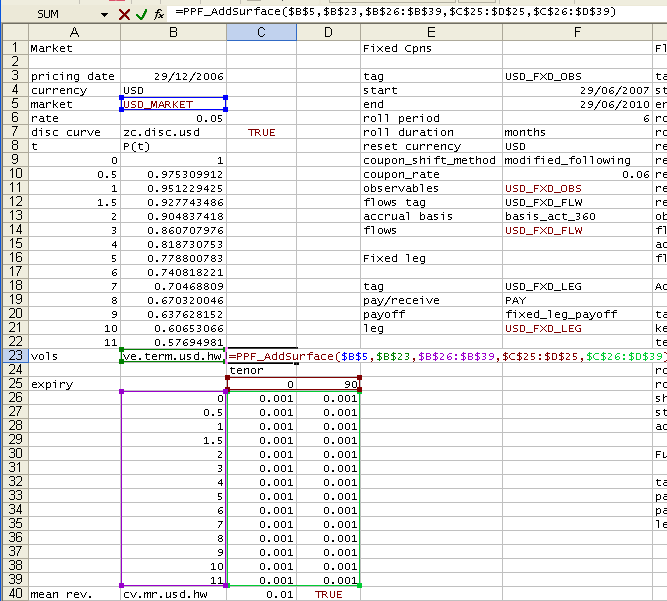
\includegraphics[scale=0.5]{img/market_server.PNG}
\caption{Adding a surface to a market environment.}
\label{fig:add-surface-to-market}
\end{figure}

\subsubsection{Market VBA client}

The foregoing section detailed the workings of the COM object known by
the ProgID \emph{`ppf.market'}. What remains is client code on the Excel
VBA side to exercise it's functionality.

It seems fair to assume that readers with interest in this chapter are
familiar with Excel and Excel VBA so we will make little comment on the
example VBA code presented here.

\subsubsection{PPF\_CreateMarketEnvironment}

This function calls out to the \verb|class MarketServer|
\verb|CreateEnvironment| method to construct and register an empty
\verb|ppf.market.environment.environment| instance.
\begin{verbatim}
Public Function _
PPF_CreateMarketEnvironment( _
    Tag As String _
  , T As Date) As String
'Create a ppf market data environment
'
On Error Resume Next
  Dim MarketServer As Object
  Set MarketServer = CreateObject("ppf.market")
  PPF_CreateMarketEnvironment = MarketServer.CreateEnvironment(Tag, T)
  If Err.Number <> 0 Then
    PPF_CreateMarketEnvironment = "#err: " & Err.Description
  End If
  Set MarketServer = Nothing
End Function
\end{verbatim}

\subsubsection{PPF\_AddCurve}

This function calls out to the \verb|class MarketServer|
\verb|AddCurve| method to register a user defined curve in a
previously constructed environment.
\begin{verbatim}
Public Function _
PPF_AddCurve( _
    Market As String _
  , Name As String _
  , Curve As Variant _
  , Interp As String) As Variant
  'Add a curve to a ppf market data environment
  '
  On Error Resume Next
  Dim MarketServer As Object
  Dim N As Integer: N = Curve.Rows.Count
  If Curve.Columns.Count <> 2 Then
    PPF_AddCurve = "#err: invalid argument"
    Exit Function
  End If
  Dim V As Variant
  ReDim V(N, 2)
  Dim I As Integer
  For I = 1 To N
    V(I, 1) = Curve(I, 1).Value
    V(I, 2) = Curve(I, 2).Value
  Next I
  Set MarketServer = CreateObject("ppf.market")
  Call MarketServer.AddCurve(Market, Name, V, Interp)
  If Err.Number <> 0 Then
    PPF_AddCurve = "#err: " & Err.Description
  Else
    PPF_AddCurve = True
  End If
  Set MarketServer = Nothing
End Function
\end{verbatim}

\subsubsection{PPF\_AddConstant}
This function calls out to the \verb|class MarketServer|
\verb|AddConstant| method to register a user constant in a previously
constructed environment.
\begin{verbatim}
Public Function _
PPF_AddConstant( _
    Market As String _
  , Name As String _
  , Value As Double) As Variant
  'Add a constant to a ppf market data environment
  '
  On Error Resume Next
  Dim MarketServer As Object
  Set MarketServer = CreateObject("ppf.market")
  Call MarketServer.AddConstant(Market, Name, Value)
  If Err.Number <> 0 Then
    PPF_AddConstant = "#err: " & Err.Description
  Else
    PPF_AddConstant = True
  End If
  Set MarketServer = Nothing
End Function
\end{verbatim}

\subsubsection{PPF\_AddSurface}
This function calls out to the \verb|class MarketServer|
\verb|AddSurface| method to register a user defined surface in a previously
constructed environment.
\begin{verbatim}
Public Function _
PPF_AddSurface( _
    Market As String _
  , Name As String _
  , Expiries As Variant _
  , Tenors As Variant _
  , Surface As Variant)
  'Add a surface to a ppf market data environment
  '
  On Error Resume Next
  Dim NumExp As Integer: NumExp = Expiries.Rows.Count
  Dim NumTen As Integer: NumTen = Tenors.Columns.Count
  If Surface.Rows.Count <> NumExp Or _
     Surface.Columns.Count <> NumTen Then
    PPF_AddSurface = "#err: invalid argument"
  End If
  Dim Exp As Variant
  ReDim Exp(NumExp)
  Dim I, J As Integer
  For I = 1 To NumExp
    Exp(I) = Expiries(I).Value
  Next I
  Dim Ten As Variant
  ReDim Ten(NumTen)
  For I = 1 To NumTen
    Ten(I) = Tenors(1, I).Value
  Next I
  Dim Values As Variant
  ReDim Values(NumExp, NumTen)
  For I = 1 To NumExp
    For J = 1 To NumTen
        Values(I, J) = Surface(I, J).Value
    Next J
  Next I
  Dim MarketServer As Object
  Set MarketServer = CreateObject("ppf.market")
  Call MarketServer.AddSurface(Market, Name, Exp, Ten, Values)
  If Err.Number <> 0 Then
    PPF_AddSurface = "#err : " & Err.Description
  Else
    PPF_AddSurface = True
  End If
  Set MarketServer = Nothing
End Function
\end{verbatim}

\subsection{Trade Server}

Having constructed a market, the next step in numerical pricing is to
describe the trade to be priced. This section outlines the 
\verb|class TradeServer| COM component. The code in this section can be found in
the \verb|ppf.com.trade_server| module. Instances of this type wrap
the services offered up by the \verb|ppf.core| module, specifically,
those relating to the \verb|ppf| trade data model (this functionality
was explained in chapter \ref{ch:data-model}). Here we go with the code:
\begin{verbatim}
import ppf.core
import ppf.pricer.payoffs
import ppf.date_time
import utils

class TradeServer(object):
  _reg_progid_ = "ppf.trade"
  _reg_clsid_ = "{E33DA322-B011-4FE9-8AB9-87A964EDD046}"
  _public_methods_ = \
   [
        "GenerateFixedCouponObservables"
            , "GenerateLiborObservables"
                       , "GenerateFlows"
               , "GenerateAdjuvantTable"
            , "GenerateExerciseSchedule"
                           , "CreateLeg"
                         , "CreateTrade"
  ]
  _observables = {}
  _flows       = {}
  _adjuvants   = {}
  _legs        = {}
  _exercises   = {}
  _trades      = {}

  retrieve = staticmethod(
       lambda tag, which :
         utils.retrieve('trade_server', 'TradeServer', tag, which))

  def GenerateFixedCouponObservables(
      self
      , tag
      , start
      , end
      , roll_period
      , roll_duration
      , reset_currency
      , coupon_shift_method
      , coupon_rate):
    try:
      observables = \
       ppf.core.generate_fixed_coupon_observables(
            start=utils.to_ppf_date(start)
          , end=utils.to_ppf_date(end)
          , roll_period=roll_period
          , roll_duration=eval("ppf.date_time."+roll_duration)
          , reset_currency=reset_currency
          , coupon_shift_method=
              eval("ppf.date_time.shift_convention."+coupon_shift_method)
          , coupon_rate=coupon_rate)
      TradeServer._observables[tag] = observables
      return tag
    except RuntimeError, e: utils.raise_com_exception(e)

  def GenerateLiborObservables(
      self
      , tag
      , start
      , end
      , roll_period
      , roll_duration
      , reset_period
      , reset_duration
      , reset_currency
      , reset_basis
      , reset_shift_method):
    try:
      observables = \
        ppf.core.generate_libor_observables(
            start=utils.to_ppf_date(start)
          , end=utils.to_ppf_date(end)
          , roll_period=roll_period
          , roll_duration = eval("ppf.date_time."+roll_duration)
          , reset_period = reset_period
          , reset_duration = eval("ppf.date_time."+reset_duration)
          , tenor_period = reset_period
          , tenor_duration = eval("ppf.date_time."+reset_duration)
          , reset_currency=reset_currency
          , reset_basis = eval("ppf.date_time."+reset_basis)
          , reset_shift_method=eval( \
             "ppf.date_time.shift_convention."+reset_shift_method)
          , reset_lag = 0)
      TradeServer._observables[tag] = observables
      return tag
    except RuntimeError, e: utils.raise_com_exception(e)

  def GenerateFlows(
      self
      , tag
      , start
      , end
      , period
      , duration
      , pay_currency
      , pay_shift_method
      , accrual_basis
      , observables):
    try:
      flows = ppf.core.generate_flows(
          start=utils.to_ppf_date(start)
          , end=utils.to_ppf_date(end)
          , duration=eval("ppf.date_time."+duration)
          , period=period
          , pay_shift_method=eval(\
              "ppf.date_time.shift_convention."+pay_shift_method)
          , pay_currency=pay_currency
          , accrual_basis=eval("ppf.date_time."+accrual_basis)
          , observables=TradeServer.retrieve(observables, 'observables'))
      TradeServer._flows[tag] = flows
      return tag
    except RuntimeError, e: utils.raise_com_exception(e)

  def GenerateAdjuvantTable(
      self
      , tag
      , items
      , tens
      , vals
      , start
      , roll_period
      , roll_duration
      , shift_method):
    try:
      import numpy
      adjuvants = \
         ppf.core.generate_adjuvant_table(
              items[1:]
            , [int(t) for t in tens[1:]]
            , numpy.array([x[1:len(vals[0])] for x in vals[1:]])
            , utils.to_ppf_date(start)
            , rol_period=roll_period
            , roll_duration=eval("ppf.date_time."+roll_duration)
            , shift_method=eval(\
                 "ppf.date_time.shift_convention."+shift_method))
      TradeServer._adjuvants[tag] = adjuvants
      return tag
    except RuntimeError, e: utils.raise_com_exception(e)

  def GenerateExerciseSchedule(
      self
      , tag
      , start
      , end
      , period
      , duration
      , shift_method):
    try:
      sched = \
        ppf.core.generate_exercise_table(
            start = utils.to_ppf_date(start)
          , end = utils.to_ppf_date(end)
          , period = period
          , duration = eval("ppf.date_time."+duration)
          , shift_method = eval("ppf.date_time.shift_convention."+shift_method))
      TradeServer._exercises[tag] = sched
      return tag
    except RuntimeError, e:
      utils.raise_com_exception(e)
    
  def CreateLeg(
    self
    , tag
    , flows
    , pay_or_receive
    , adjuvant_table
    , payoff):
    try:
      adjuvants = None
      if adjuvant_table:
        adjuvants = TradeServer.retrieve(adjuvant_table, 'adjuvants')
      leg = \
          ppf.core.leg(
             TradeServer.retrieve(flows, 'flows')
             , eval("ppf.core."+pay_or_receive)
             , adjuvants
             , eval("ppf.pricer.payoffs."+payoff)())
      TradeServer._legs[tag] = leg
      return tag
    except RuntimeError, e: utils.raise_com_exception(e)

  def CreateTrade(
    self
    , tag
    , legs
    , exercise_sched
    , exercise_type):
    try:
      tl = [TradeServer.retrieve(l, 'legs') for l in legs[1:]]
      if exercise_sched:
        exercises = TradeServer.retrieve(exercise_sched, 'exercises')
        if not exercise_type:
          raise RuntimeError, "missing exercise type"
        call_cancel = eval("ppf.core.exercise_type."+exercise_type)
        trade = ppf.core.trade(tl, (exercises, call_cancel))
      else:
        trade = ppf.core.trade(tl, None)
      TradeServer._trades[tag] = trade
      return tag
    except RuntimeError, e: utils.raise_com_exception(e)
    
if __name__ == "__main__": utils.register_com_class(TradeServer)
\end{verbatim}

Sub-section \ref{subsec:market-server} covers the details of what
needs to be known to `technically' understand the above code so this
section need not be so detailed from that perspective.

As is the case for \verb|class MarketServer|, the \verb|class TradeServer|
implementation follows a `mono-state' idiom. Unlike, 
\verb|class MarketServer|, however, \verb|class TradeServer| maintains
multiple dictionaries in its class object state
\begin{verbatim}
  _observables = {} #observable collections
  _flows       = {} #flow collections
  _adjuvants   = {} #adjuvant tables
  _legs        = {} #trade legs
  _exercises   = {} #exercise schedules
  _trades      = {} #trades
\end{verbatim}
As for \verb|class MarketServer|, \verb|class TradeServer| offers a
static method for inter-module retrieval of data from these
dictionaries. 

As for the COM interface, \verb|GenerateFixedCouponObservables| rolls
out strips of fixed coupons, whereas
\verb|GenerateLiborCouponObservables| rolls out strips of LIBORs (it's
left as an exercise to the reader to write the function that rolls out
strips of swap rate observables). \verb|GenerateFlows| rolls out flows
with observable collections folded in. \verb|GenerateAdjuvantTable|
and \\
\verb|GenerateExerciseSchedule| provide the means of constructing
adjuvant tables (refer to section \ref{sec:adjuvant-tables}) and
exercise schedules respectively. Finally, \verb|CreateLeg| assembles a
flow collection, a user provided payoff string and potentially an
adjuvant table into a trade leg (the payoff string needs to map to a
class name in the \verb|ppf.pricer.payoffs| module
such as, \verb|fixed_leg_payoff|, \verb|float_leg_payoff| for
example). Finally, legs and perhaps an associated exercise schedule
can be aggregated into trades with the \verb|CreateTrade| method. Figure
\ref{fig:create-trade} shows how the data for describing a Bermudan
swaption might be laid out in an Excel worksheet.
\begin{figure} 
\centering
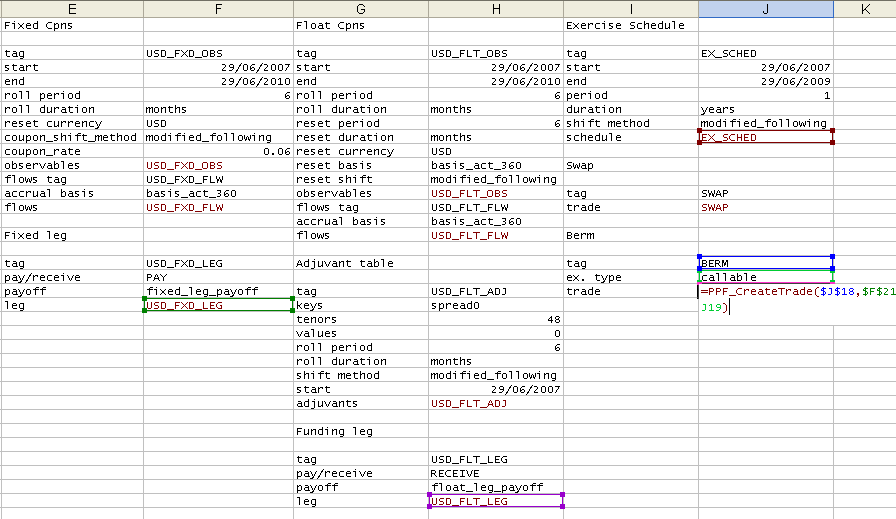
\includegraphics[scale=0.4]{img/trade_server.PNG}
\caption{Creating a Bermudan swaption.}
\label{fig:create-trade}
\end{figure}

\subsubsection{Trade VBA client}

Here is example client code for interfacing to the
\emph{`ppf.trade'} COM object.

\subsubsection{PPF\_GenerateFixedCouponObservables}

This function calls out to the \verb|class TradeServer|
\verb|GenerateFixedCouponObservables| method to create and register
observables to underly a fixed trade leg.

\begin{verbatim}
Public Function _
PPF_GenerateFixedCouponObservables( _
    Tag As String _
  , Begin As Date _
  , Finish As Date _
  , Period As Integer _
  , Duration As String _
  , Ccy As String _
  , Shift As String _
  , Rate As Double) As String
  'Generate a ppf fixed coupon observable sequence
  '
  On Error Resume Next
  Dim TradeServer As Object
  Set TradeServer = CreateObject("ppf.trade")
  PPF_GenerateFixedCouponObservables = _
    TradeServer.GenerateFixedCouponObservables( _
        Tag _
      , Begin _
      , Finish _
      , Period _
      , Duration _
      , Ccy _
      , Shift _
      , Rate)
  If Err.Number <> 0 Then
    PPF_GenerateFixedCouponObservables = "#err : " & Err.Description
  End If
  Set TradeServer = Nothing
End Function
\end{verbatim}

\subsubsection{PPF\_GenerateLiborObservables}

This function calls out to the \verb|class TradeServer|
\verb|GenerateLiborObservables| method to create and register the
observables to underly a funding trade leg.
\begin{verbatim}
Public Function _
PPF_GenerateLiborObservables( _
    Tag As String _
  , Begin As Date _
  , Finish As Date _
  , RollPeriod As Integer _
  , RollDuration As String _
  , ResetPeriod As Integer _
  , ResetDuration As String _
  , ResetCcy As String _
  , ResetBasis As String _
  , ResetShift As String) As String
  'Generate a ppf libor observable sequence
  '
  On Error Resume Next
  Dim TradeServer As Object
  Set TradeServer = CreateObject("ppf.trade")
  PPF_GenerateLiborObservables = _
    TradeServer.GenerateLiborObservables( _
        Tag _
      , Begin _
      , Finish _
      , RollPeriod _
      , RollDuration _
      , ResetPeriod _
      , ResetDuration _
      , ResetCcy _
      , ResetBasis _
      , ResetShift)
  If Err.Number <> 0 Then
    PPF_GenerateLiborObservables = "#err : " & Err.Description
  End If
  Set TradeServer = Nothing
End Function
\end{verbatim}

\subsubsection{PPF\_GenerateAdjuvantTable}

This function calls out to the \verb|class TradeServer|
\verb|GenerateAdjuvantTable| method to build and register an
adjuvant table.
\begin{verbatim}
Public Function _
PPF_GenerateAdjuvantTable( _
    Tag As String _
  , Items As Variant _
  , Tenors As Variant _
  , Values As Variant _
  , Start As Date _
  , RollPeriod As Integer _
  , RollDuration As String _
  , ShiftConv As String) As String
  'Generate a ppf adjuvant table
  '
  On Error Resume Next
  Dim TradeServer As Object
  Set TradeServer = CreateObject("ppf.trade")
  Dim K As Integer
  K = Items.Rows.Count
  If Items.Columns.Count <> 1 Then
   PPF_GenerateAdjuvantTable = "#err : " & "invalid argument"
   Exit Function
  End If
  Dim Keys As Variant
  ReDim Keys(K)
  Dim I, J As Integer
  For I = 1 To K
    Keys(I) = Items(I).Value
  Next I
  Dim M, N As Integer
  M = Values.Rows.Count
  N = Values.Columns.Count
  If M <> K Then
   PPF_GenerateAdjuvantTable = "#err : " & "invalid argument"
   Exit Function
  End If
  Dim Vals As Variant
  ReDim Vals(M, N)
  For I = 1 To M
    For J = 1 To N
        Vals(I, J) = Values(I, J).Value
    Next J
  Next I
  If Tenors.Rows.Count > 1 Or Tenors.Columns.Count <> N Then
   PPF_GenerateAdjuvantTable = "#err : " & "invalid argument"
   Exit Function
  End If
  Dim Tens As Variant
  ReDim Tens(N)
  For J = 1 To N
    Tens(J) = Tenors(J).Value
  Next J
  PPF_GenerateAdjuvantTable = _
    TradeServer.GenerateAdjuvantTable( _
        Tag _
      , Keys _
      , Tens _
      , Vals _
      , Start _
      , RollPeriod _
      , RollDuration _
      , ShiftConv)
  If Err.Number <> 0 Then
    PPF_GenerateAdjuvantTable = "#err : " & Err.Description
  End If
  Set TradeServer = Nothing

End Function
\end{verbatim}

\subsubsection{PPF\_GenerateFlows}

This function calls out to the \verb|class TradeServer|
\verb|GenerateFlows| method to create and register a flow collection.
\begin{verbatim}
Public Function _
PPF_GenerateFlows( _
    Tag As String _
  , Begin As Date _
  , Finish As Date _
  , Period As Integer _
  , Duration As String _
  , Ccy As String _
  , Shift As String _
  , Basis As String _
  , Observables As String) As String
  'Generate a ppf flow sequence
  '
  On Error Resume Next
  Dim TradeServer As Object
  Set TradeServer = CreateObject("ppf.trade")
  PPF_GenerateFlows = _
    TradeServer.GenerateFlows( _
        Tag _
      , Begin _
      , Finish _
      , Period _
      , Duration _
      , Ccy _
      , Shift _
      , Basis _
      , Observables)
  If Err.Number <> 0 Then
    PPF_GenerateFlows = "#err : " & Err.Description
  End If
  Set TradeServer = Nothing
End Function
\end{verbatim}

\subsubsection{PPF\_GenerateExerciseSchedule}

This function calls out to the \verb|class TradeServer|
\verb|GenerateExerciseSchedule| method to create and register an
exercise schedule.
\begin{verbatim}
Public Function _
PPF_GenerateExerciseSchedule( _
    Tag As String _
  , Begin As Date _
  , Finish As Date _
  , Period As Integer _
  , Duration As String _
  , Shift As String) As String
  'Generate a ppf exercise schedule
  '
  On Error Resume Next
  Dim TradeServer As Object
  Set TradeServer = CreateObject("ppf.trade")
  PPF_GenerateExerciseSchedule = _
    TradeServer.GenerateExerciseSchedule( _
        Tag _
      , Begin _
      , Finish _
      , Period _
      , Duration _
      , Shift)
  If Err.Number <> 0 Then
    PPF_GenerateExerciseSchedule = "#err : " & Err.Description
  End If
  Set TradeServer = Nothing
End Function
\end{verbatim}

\subsubsection{PPF\_CreateLeg}

This function calls out to the \verb|class TradeServer|
\verb|CreateLeg| function to create and register a trade leg.
\begin{verbatim}
Public Function _
PPF_CreateLeg( _
    Tag As String _
  , Flows As String _
  , PayOrReceive As String _
  , AdjuvantTable As Variant _
  , Payoff As String) As String
  'Create a ppf trade leg
  '
  On Error Resume Next
  Dim TradeServer As Object
  Set TradeServer = CreateObject("ppf.trade")
  If IsMissing(AdjuvantTable) Then
    PPF_CreateLeg = _
      TradeServer.CreateLeg( _
          Tag _
        , Flows _
        , PayOrReceive _
        , Nothing _
        , Payoff)
  Else
    PPF_CreateLeg = _
      TradeServer.CreateLeg( _
          Tag _
        , Flows _
        , PayOrReceive _
        , CStr(AdjuvantTable) _
        , Payoff)
  End If
  If Err.Number <> 0 Then
    PPF_CreateLeg = "#err : " & Err.Description
  End If
  Set TradeServer = Nothing

End Function
\end{verbatim}

\subsubsection{PPF\_CreateTrade}

This function calls out to the \verb|class TradeServer|
\verb|CreateTrade| method to create and register a trade.
\begin{verbatim}
Public Function _
PPF_CreateTrade( _
    Tag As String _
  , Leg1 As String _
  , Leg2 As String _
  , ExerciseSched As Variant _
  , ExerciseType As Variant) As String
  'Create a ppf trade
  '
  On Error Resume Next
  Dim TradeServer As Object
  Set TradeServer = CreateObject("ppf.trade")
  Dim Legs(2) As String
  Legs(1) = Leg1: Legs(2) = Leg2
  If IsMissing(ExerciseSched) Then
    PPF_CreateTrade = _
      TradeServer.CreateTrade( _
          Tag _
        , Legs _
        , Nothing _
        , Nothing)
  Else
    PPF_CreateTrade = _
      TradeServer.CreateTrade( _
          Tag _
        , Legs _
        , CStr(ExerciseSched) _
        , CStr(ExerciseType))
  End If
  If Err.Number <> 0 Then
    PPF_CreateTrade = "#err : " & Err.Description
  End If
  Set TradeServer = Nothing
End Function
\end{verbatim}

\subsection{Pricer Server}\label{subsec:pricer-server}

We are very close to achieving the goal as stated in the opening to
this section, that is, pricing Bermudans on a Hull-White lattice from
Excel.

The last component to consider is the \verb|class PricerServer| the
code for which can be found in the \verb|ppf.com.pricer_server|
module:
\begin{verbatim}
import ppf.model
import ppf.pricer
import utils

class PricerServer(object):
  _reg_progid_ = "ppf.pricer"
  _reg_clsid_ = "{08632905-0B63-45B5-B388-30C73CAE611C}"
  _public_methods_ = \
  [
      "CreateHullWhiteLatticePricer"
                    , "InvokePricer"
  ]
  _pricers = {}

  retrieve = staticmethod(
       lambda tag, which :
         utils.retrieve('pricer_server', 'PricerServer', tag, which))

  def CreateHullWhiteLatticePricer(
      self
      , tag
      , trade_id
      , env_id
      , num_states
      , num_std_dev):
    try:
      from trade_server import TradeServer
      from market_server import MarketServer
      trade = TradeServer.retrieve(trade_id, 'trades')
      env   = MarketServer.retrieve(env_id, 'environments')
      model_args = {"num states": num_states, "num std dev": num_std_dev} 
      factory = ppf.model.hull_white_lattice_model_factory()
      model = factory(trade, env, model_args)
      pricer = ppf.pricer.lattice_pricer(trade, model, env, None)
      PricerServer._pricers[tag] = pricer
      return tag
    except RuntimeError, e: ppf.com.utils.raise_com_exception(e)

  def InvokePricer(self, tag):
    try:
      return PricerServer.retrieve(tag, 'pricers').__call__()
    except RuntimeError, e: utils.raise_com_exception(e)

if __name__ == "__main__": utils.register_com_class(PricerServer)
\end{verbatim}
The explanations provided by the earlier sections should make the
above code self-explanatory rendering further comment unnecessary.
Figure \ref{fig:price-bermudan} shows an example session pricing a
Bermudan in an Excel session.
\begin{figure} \centering
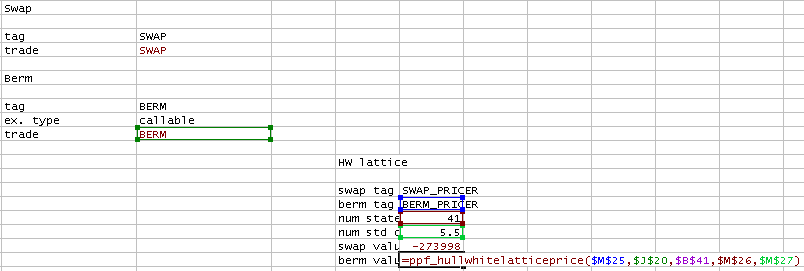
\includegraphics[scale=0.5]{img/pricer_server.PNG}
\caption{Pricing a berm.}
\label{fig:price-bermudan}
\end{figure}

\subsubsection{Pricer VBA client}

Here is the example client code for interfacing to the
\emph{`ppf.pricer'} COM object.

\subsubsection{PPF\_HullWhiteLatticePrice}

The function for obtaining the price of a trade via the Hull-White
model on a lattice.

\begin{verbatim}
Public Function _
PPF_HullWhiteLatticePrice( _
    Tag As String _
  , trade As String _
  , Env As String _
  , NumStates As Integer _
  , NumStdDevs As Double) As Variant
  'Price trade on a Hull-White lattice
  '
  On Error Resume Next
  Dim PricerServer As Object
  Set PricerServer = CreateObject("ppf.pricer")
  PPF_HullWhiteLatticePrice = _
    PricerServer.InvokePricer( _
      PricerServer.CreateHullWhiteLatticePricer( _
          Tag _
        , trade _
        , Env _
        , NumStates _
        , NumStdDevs))
  If Err.Number <> 0 Then
    PPF_HullWhiteLatticePrice = "#err : " & Err.Description
  End If
  Set PricerServer = Nothing
End Function
\end{verbatim}
